\documentclass{standalone}
\usepackage{tikz}
\usetikzlibrary{patterns, positioning}


\begin{document}
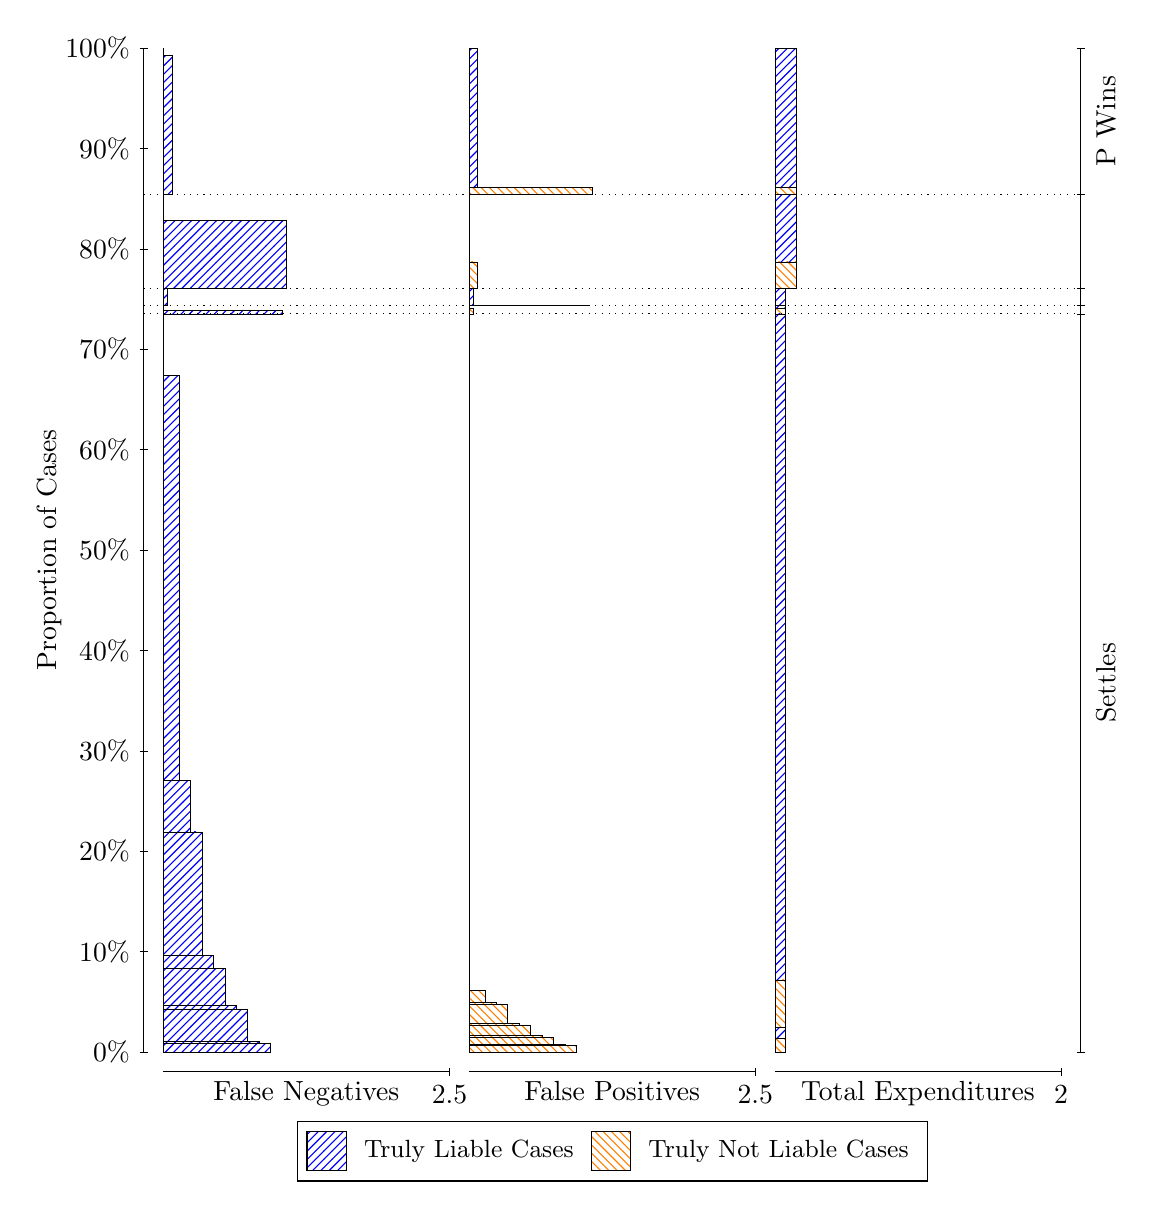
\begin{tikzpicture}
\draw[black, very thin] (1.5,1.75) -- (1.5,14.5);
\node[rotate=90, text=black, anchor=center] at (0.3, 8.125) {Proportion of Cases};
\draw[black, very thin] (1.45,1.75) -- (1.55,1.75);
\node[text=black, anchor=east] at (1.45, 1.75) {0\%};
\draw[black, very thin] (1.45,3.025) -- (1.55,3.025);
\node[text=black, anchor=east] at (1.45, 3.025) {10\%};
\draw[black, very thin] (1.45,4.3) -- (1.55,4.3);
\node[text=black, anchor=east] at (1.45, 4.3) {20\%};
\draw[black, very thin] (1.45,5.575) -- (1.55,5.575);
\node[text=black, anchor=east] at (1.45, 5.575) {30\%};
\draw[black, very thin] (1.45,6.85) -- (1.55,6.85);
\node[text=black, anchor=east] at (1.45, 6.85) {40\%};
\draw[black, very thin] (1.45,8.125) -- (1.55,8.125);
\node[text=black, anchor=east] at (1.45, 8.125) {50\%};
\draw[black, very thin] (1.45,9.4) -- (1.55,9.4);
\node[text=black, anchor=east] at (1.45, 9.4) {60\%};
\draw[black, very thin] (1.45,10.675) -- (1.55,10.675);
\node[text=black, anchor=east] at (1.45, 10.675) {70\%};
\draw[black, very thin] (1.45,11.95) -- (1.55,11.95);
\node[text=black, anchor=east] at (1.45, 11.95) {80\%};
\draw[black, very thin] (1.45,13.225) -- (1.55,13.225);
\node[text=black, anchor=east] at (1.45, 13.225) {90\%};
\draw[black, very thin] (1.45,14.5) -- (1.55,14.5);
\node[text=black, anchor=east] at (1.45, 14.5) {100\%};

\draw[black, very thin] (13.4,1.75) -- (13.4,14.5);
\draw[black, very thin] (13.35,1.75) -- (13.45,1.75);
\node[anchor=west] at (13.35, 1.75) {};
\draw[black, very thin] (13.35,11.124) -- (13.45,11.124);
\node[anchor=west] at (13.35, 11.124) {};
\draw[black, very thin] (13.35,11.23) -- (13.45,11.23);
\node[anchor=west] at (13.35, 11.23) {};
\draw[black, very thin] (13.35,11.451) -- (13.45,11.451);
\node[anchor=west] at (13.35, 11.451) {};
\draw[black, very thin] (13.35,12.64) -- (13.45,12.64);
\node[anchor=west] at (13.35, 12.64) {};
\draw[black, very thin] (13.35,14.5) -- (13.45,14.5);
\node[anchor=west] at (13.35, 14.5) {};

\draw[black, very thin, pattern color=blue, pattern=north east lines] (1.75,1.75) rectangle (3.1125,1.8601);
\draw[black, very thin, pattern color=blue, pattern=north east lines] (1.75,1.8601) rectangle (2.9672,1.8849);
\draw[black, very thin, pattern color=blue, pattern=north east lines] (1.75,1.8849) rectangle (2.8218,2.2865);
\draw[black, very thin, pattern color=blue, pattern=north east lines] (1.75,2.2865) rectangle (2.6765,2.3411);
\draw[black, very thin, pattern color=blue, pattern=north east lines] (1.75,2.3411) rectangle (2.5312,2.814);
\draw[black, very thin, pattern color=blue, pattern=north east lines] (1.75,2.814) rectangle (2.3858,2.9768);
\draw[black, very thin, pattern color=blue, pattern=north east lines] (1.75,2.9768) rectangle (2.2405,4.5462);
\draw[black, very thin, pattern color=blue, pattern=north east lines] (1.75,4.5462) rectangle (2.0952,5.1946);
\draw[black, very thin, pattern color=blue, pattern=north east lines] (1.75,5.1946) rectangle (1.9498,10.345);
\draw[black, very thin, pattern color=orange, pattern=north west lines] (1.75,10.345) rectangle (1.75,11.124);
\draw[black, very thin, pattern color=blue, pattern=north east lines] (1.75,11.124) rectangle (3.2578,11.164);
\draw[black, very thin, pattern color=orange, pattern=north west lines] (1.75,11.164) rectangle (1.75,11.23);
\draw[black, very thin, pattern color=blue, pattern=north east lines] (1.75,11.23) rectangle (1.8045,11.449);
\draw[black, very thin, pattern color=orange, pattern=north west lines] (1.75,11.449) rectangle (1.75,11.451);
\draw[black, very thin, pattern color=blue, pattern=north east lines] (1.75,11.451) rectangle (3.3123,12.308);
\draw[black, very thin, pattern color=orange, pattern=north west lines] (1.75,12.308) rectangle (1.75,12.64);
\draw[black, very thin, pattern color=blue, pattern=north east lines] (1.75,12.64) rectangle (1.859,14.405);
\draw[black, very thin, pattern color=orange, pattern=north west lines] (1.75,14.405) rectangle (1.75,14.5);
\draw[black, very thin, pattern color=orange, pattern=north west lines] (5.6333,1.75) rectangle (6.9958,1.831);
\draw[black, very thin, pattern color=orange, pattern=north west lines] (5.6333,1.831) rectangle (6.8505,1.8416);
\draw[black, very thin, pattern color=orange, pattern=north west lines] (5.6333,1.8416) rectangle (6.7052,1.9391);
\draw[black, very thin, pattern color=orange, pattern=north west lines] (5.6333,1.9391) rectangle (6.5598,1.956);
\draw[black, very thin, pattern color=orange, pattern=north west lines] (5.6333,1.956) rectangle (6.4145,2.0896);
\draw[black, very thin, pattern color=orange, pattern=north west lines] (5.6333,2.0896) rectangle (6.2692,2.1135);
\draw[black, very thin, pattern color=orange, pattern=north west lines] (5.6333,2.1135) rectangle (6.1238,2.3541);
\draw[black, very thin, pattern color=orange, pattern=north west lines] (5.6333,2.3541) rectangle (5.9785,2.3797);
\draw[black, very thin, pattern color=orange, pattern=north west lines] (5.6333,2.3797) rectangle (5.8332,2.5296);
\draw[black, very thin, pattern color=blue, pattern=north east lines] (5.6333,2.5296) rectangle (5.6333,11.124);
\draw[black, very thin, pattern color=orange, pattern=north west lines] (5.6333,11.124) rectangle (5.6878,11.19);
\draw[black, very thin, pattern color=blue, pattern=north east lines] (5.6333,11.19) rectangle (5.6333,11.23);
\draw[black, very thin, pattern color=orange, pattern=north west lines] (5.6333,11.23) rectangle (7.1412,11.233);
\draw[black, very thin, pattern color=blue, pattern=north east lines] (5.6333,11.233) rectangle (5.6878,11.451);
\draw[black, very thin, pattern color=orange, pattern=north west lines] (5.6333,11.451) rectangle (5.7423,11.784);
\draw[black, very thin, pattern color=blue, pattern=north east lines] (5.6333,11.784) rectangle (5.6333,12.64);
\draw[black, very thin, pattern color=orange, pattern=north west lines] (5.6333,12.64) rectangle (7.1957,12.735);
\draw[black, very thin, pattern color=blue, pattern=north east lines] (5.6333,12.735) rectangle (5.7423,14.5);
\draw[black, very thin, pattern color=orange, pattern=north west lines] (9.5167,1.75) rectangle (9.6529,1.9254);
\draw[black, very thin, pattern color=blue, pattern=north east lines] (9.5167,1.9254) rectangle (9.6529,2.0603);
\draw[black, very thin, pattern color=orange, pattern=north west lines] (9.5167,2.0603) rectangle (9.6529,2.6645);
\draw[black, very thin, pattern color=blue, pattern=north east lines] (9.5167,2.6645) rectangle (9.6529,11.124);
\draw[black, very thin, pattern color=orange, pattern=north west lines] (9.5167,11.124) rectangle (9.6529,11.19);
\draw[black, very thin, pattern color=blue, pattern=north east lines] (9.5167,11.19) rectangle (9.6529,11.23);
\draw[black, very thin, pattern color=orange, pattern=north west lines] (9.5167,11.23) rectangle (9.6529,11.233);
\draw[black, very thin, pattern color=blue, pattern=north east lines] (9.5167,11.233) rectangle (9.6529,11.451);
\draw[black, very thin, pattern color=orange, pattern=north west lines] (9.5167,11.451) rectangle (9.7892,11.784);
\draw[black, very thin, pattern color=blue, pattern=north east lines] (9.5167,11.784) rectangle (9.7892,12.64);
\draw[black, very thin, pattern color=orange, pattern=north west lines] (9.5167,12.64) rectangle (9.7892,12.735);
\draw[black, very thin, pattern color=blue, pattern=north east lines] (9.5167,12.735) rectangle (9.7892,14.5);
\draw[black, dotted] (1.5,11.124) -- (13.4,11.124);
\draw[black, dotted] (1.5,11.23) -- (13.4,11.23);
\draw[black, dotted] (1.5,11.451) -- (13.4,11.451);
\draw[black, dotted] (1.5,12.64) -- (13.4,12.64);
\draw[black, very thin] (1.75,1.5) -- (5.3833,1.5);
\node[text=black, anchor=north] at (3.5667, 1.5) {False Negatives};
\draw[black, very thin] (5.3833,1.45) -- (5.3833,1.55);
\node[text=black, anchor=north] at (5.3833, 1.45) {2.5};

\draw[black, very thin] (5.6333,1.5) -- (9.2667,1.5);
\node[text=black, anchor=north] at (7.45, 1.5) {False Positives};
\draw[black, very thin] (9.2667,1.45) -- (9.2667,1.55);
\node[text=black, anchor=north] at (9.2667, 1.45) {2.5};

\draw[black, very thin] (9.5167,1.5) -- (13.15,1.5);
\node[text=black, anchor=north] at (11.333, 1.5) {Total Expenditures};
\draw[black, very thin] (13.15,1.45) -- (13.15,1.55);
\node[text=black, anchor=north] at (13.15, 1.45) {2};

\node[text=black, centered, rotate=90] at (13.72, 6.4371) {Settles};



\node[text=black, centered, rotate=90] at (13.72, 13.57) {P Wins};

\draw (7.449999999999999,1.5) node[draw=none] (baseCoordinate) {};
\begin{scope}[align=center]
        \matrix[scale=0.5, draw=black, below=0.5cm of baseCoordinate, nodes={draw}, column sep=0.1cm]{
            \node[rectangle, draw, minimum width=0.5cm, minimum height=0.5cm, pattern color=blue, pattern=north east lines] {}; &
            \node[draw=none, font=\small, text=black] (B) {Truly Liable Cases}; &
            \node[rectangle, draw, minimum width=0.5cm, minimum height=0.5cm, pattern color=orange, pattern=north west lines] {}; &
            \node[draw=none, font=\small, text=black] (B) {Truly Not Liable Cases}; \\
            };
\end{scope}

\end{tikzpicture}
\end{document}